
\newpage
\changefontsizes{16pt}
\centerline{\textbf{CHƯƠNG I: CÁC MÔ HÌNH}}
\centerline{\textbf{TIME SERIES FORECASTING}}

\vspace{1.2cm}
\changefontsizes{13pt}
\setlength{\parindent}{0cm}
Từ trước đến nay, việc xem xét, đánh giá những khả năng có thể xảy ra và tác động của nó đến các công ty, tổ chức, bộ máy là một điều hết sức quan trọng. Điều này là nhân tố quyết định cho sự tồn tại và phát triển của các cơ quan, đoàn thể. Dĩ nhiên nó đòi hỏi có một sự tỉ mỉ, một cái nhìn bao quát, một sự tính toán trong nhiều năm trời, và chỉ dành cho những chuyên gia thâm niên, những nhà nghiên cứu tài ba trong chính lĩnh vực đó. Một công việc không ít tốn kém cả về sức người lẫn sức của.


\begin{center}
	\begin{figure}[htp]
		\begin{center}
			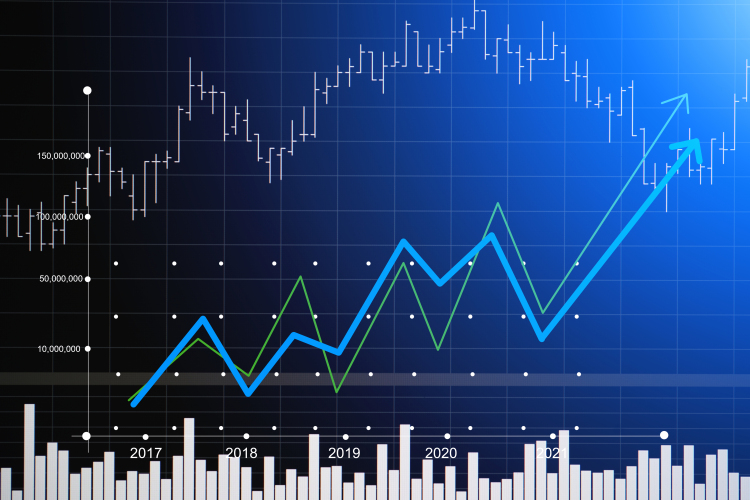
\includegraphics[scale=2.2]{./images/stock.jpg}
		\end{center}
	\end{figure}
\label{fig1}{Hình 1: Bảng thống kê sự tăng trưởng cổ phiếu (hình minh họa)}
\end{center}

Bài toán về việc sử dụng máy tính để tính toán, dự đoán tương lai, dự đoán kết quả có thể xảy ra dựa trên những dữ kiện đã ghi nhận từ quá khứ đến hiện tại, không phải là một điều gì mới mẻ. Nhưng trước đó do hiệu quả và khả năng dự đoán kém, nên bài toán này không được cộng đồng xã hội chú ý đến. Tuy nhiên, trong những năm trở lại đây, như một quả bom, nó đã bùng nổ và lan rộng khắp thế giới, đón nhận được sự quan tâm nhiệt tình của không chỉ cộng đồng khoa học mà còn cả các ngành nghề, lĩnh vực khác (kinh tế, y học, khí tượng thủy văn,...). Ấy là nhờ vào sự xuất hiện của deep learning và việc ứng dụng deep learning vào việc tính toán, đánh giá, thay đổi và cải thiện tính chính xác của bài toán.


\vspace{1cm}
\changefontsizes{15pt}
\setlength{\parindent}{0cm}
\textbf{Time series}

\vspace{1cm}
\changefontsizes{13pt}
%content
Một time series là một chuỗi dữ liệu được đánh chỉ mục (một danh sách hoặc đồ thị) theo thứ tự thời gian. Thông thường các giá trị giữ liệu được xác định/đo đạt tại các mốc thời gian cách đều nhau. Chính vì thế, time series là một chuỗi dữ liệu rời rạc. Cụ thể là các thông tin về độ ẩm, huớng gió, lực gió, lượng mây,... được đo đạt mỗi giờ tại các trạm khí tượng thủy văn.

\bigskip
Chuỗi thời gian thường được biểu diễn dưới dạng biểu đồ đường. Chúng được sử dụng trong thống kê, xử lý tín hiệu, nhận dạng mẫu, kinh tế, tài chính, toán học, dự báo thời tiết, dự báo động đất, điện não đồ, kỹ thuật điều khiển, thiên văn học, kỹ thuật truyền thông và trong bất kỳ lĩnh vực khoa học ứng dụng - kỹ thuật nào liên quan đến các phép đo thời gian.



\begin{center}
	\begin{figure}[htp]
		\begin{center}
			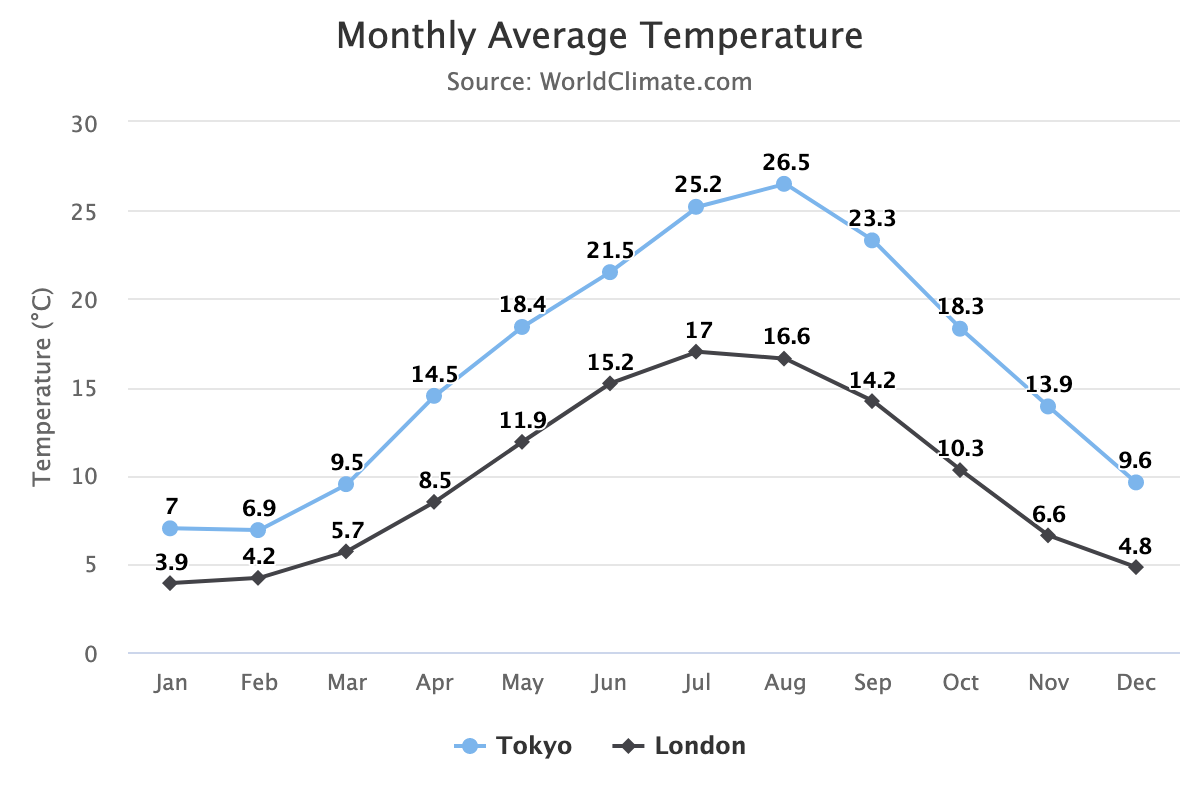
\includegraphics[scale=.3]{./images/weather.png}
		\end{center}
	\label{fig1}{Hình 2: Biểu đồ ghi lại sự thay đổi nhiệt độ của hai thành phố Tokyo và Lodon qua các tháng}
	\end{figure}
\end{center}


\bigskip
Phân tích chuỗi thời gian nhằm mục đích phát hiện và tập hợp lại các yếu tố có ảnh hưởng đến giá trị của đối tượng quan sát theo thời gian.

\bigskip
Trong Time-series Data, có hai loại chính:

- Chuỗi thời gian thông thường (regular time series), loại thông thường được gọi là số liệu.\\
- Chuỗi thời gian bất thường (events) là những sự kiện.



\vspace{1cm}
\changefontsizes{15pt}
\setlength{\parindent}{0cm}
\textbf{Time series forecasting}

\vspace{1cm}
\changefontsizes{13pt}
%content

Như đã trình bày ở trên, dự đoán dựa trên chuỗi thời gian là việc dùng những dữ liệu đã có để dự đoán sự kiện hoặc một chuỗi sự kiện có thể xảy đến trong tương lai. Tuy nhiên, dự đoán thời gian là một việc khó khăn. Không như các bài toán phân lớp và hồi quy, bài toán chuỗi thời gian làm tăng độ phức tạp của thứ tự các quan sát hay sự phụ thuộc giữa các quan sát. 

\bigskip
Người ta cũng đã dành không ít thời gian để xây dựng và điều chỉnh các mô hình, các phương pháp dự đoán thời gian sao cho sự kiện được dự đoán sai lệch thấp nhất có thể. Các phương pháp được trình bày bên dưới đây là những phương pháp phổ biến và có hiệu quả tốt nhất đã được kiểm chứng bằng thực nghiệm


\vspace{1cm}
\changefontsizes{15pt}
\setlength{\parindent}{0cm}
\textbf{Những phương pháp được sử dụng trong time series forecasting}

\bigskip
\changefontsizes{14pt}
\setlength{\parindent}{0cm}
\textbf{Phương pháp truyền thống}

\bigskip
\changefontsizes{13pt}
\setlength{\parindent}{0cm}
\textbf{Autoregressive integrated moving average (ARIMA)}

\smallskip
Mô hình trung bình trượt, đồng liên kết, tự hồi quy ARIMA sử dụng chính các giá trị trong quá khứ của Y để giải thích cho Y hiện tại. Vì việc xác định mỗi một mô hình dựa trên sự phân tích dữ liệu cụ thể cho từng trường hợp mà không phụ thuộc hay bám lấy bất kỳ một lý thuyết tổng quát nào. Nên ARIMA có được tính chất linh hoạt và tiết kiệm chi phí.

\vspace{0.7cm}
\changefontsizes{13pt}
\setlength{\parindent}{0cm}
\textbf{Hạn chế, rào cản của phương pháp truyền thống}

\begin{itemize}
	\item \textbf{Chỉ hiệu quả với dữ liệu hoàn chỉnh:} Một vài giá trị bị thiếu hụt có thể ảnh hưởng nặng nề dến mô hình.
	\item \textbf{Phụ thuộc vào mối quan hệ tuyến tính:} Các mô hình truyền thống không thích hợp với phân phối phức tạp.
	\item \textbf{Chỉ dùng được với dữ liệu đơn biến:} Trong khi thực tế, dữ liệu đầu vào hầu hết là đa biến.
	\item \textbf{Không chạy tốt với những dự đoán có chu kỳ dài:} Chúng thường chỉ tập trung vào việc dự đoán duy nhất một sự kiện (one-step).
	\item \textbf{Thời gian phụ thuộc phải là cố định:} Mối quan hệ giữa các quan sát thường luôn khác nhau tại các thời điểm khác nhau, do đó cần có sự cố định giữa các thời gian quan sát.
\end{itemize}



\vspace{0.5cm}
\changefontsizes{14pt}
\setlength{\parindent}{0cm}
\textbf{Các phương pháp mới sử dụng deep learning}


\vspace{0.25cm}
\changefontsizes{13pt}
\setlength{\parindent}{0cm}
\textbf{1. Multilayer Perceptrons (MLP)}

\bigskip
MLP có những đặt trưng nổi trội như:

\begin{itemize}
	\item Khả năng xấp xỉ các hàm phi tuyến tính. Mang lại một kết quả đầy hứa hẹn.
	\item Khả năng chịu lỗi. Học tốt kể cả khi bị thiết sót dữ liệu.
	\item Có thể xử lý dữ liệu đầu vào là đa biến.
	\item Có khả năng dự đoán nhiều bước (multi-step).
\end{itemize}



\changefontsizes{13pt}
\setlength{\parindent}{0cm}
\textbf{2. Convolutional Neural Networks (CNN)}

\bigskip
CNN thường được dùng trong việc phân lớp hình ảnh, bởi hiệu quả tuyệt vời của nó. Bên cạnh đó CNN cũng có khả năng trích xuất đặc trưng của dữ liệu đầu vào trong time series forecasting. CNN còn sở hữu đầy đủ những ưu điểm của MLP.


\vspace{0.5cm}
\changefontsizes{13pt}
\setlength{\parindent}{0cm}
\textbf{3. Recurrent Neural Networks(RNN)}

\bigskip
RNN cung cấp khả năng xử lý trật tự của các quan sát và cho phép quan sát thể hiện sự phụ thuộc theo gian của nó. Khác với MLP, RNN sử dụng chính bộ nhớ của mình để xử lý chuỗi dữ liệu đầu vào. Nhờ đó mà RNN có thể xử lý các quan sát có độ trễ cố định về thời gian. 

\vspace{0.25cm}
\changefontsizes{14pt}
\setlength{\parindent}{0cm}
\textbf{So sánh, đánh giá các phương pháp}

\changefontsizes{13pt}
%content

\begin{table}[htp]
\centering
\begin{tabular}{p{0.2\textwidth}p{0.4\textwidth}p{0.4\textwidth}}
	
\textbf{Phương pháp}            & \textbf{Ưu điểm} & \textbf{Hạn chế}  
\\
Truyền thống
&
\begin{tabular}[c]{@{}l@{}}- Đơn giản\\ - Dễ hiểu\end{tabular}
&
\begin{tabular}[c]{@{}l@{}}- Đòi hỏi dữ liệu hoàn chỉnh\\ - Chỉ có mối quan hệ tuyến tính\\- Hiệu quả với đơn biến\\- Kém hiệu quả với chu kỳ dài\end{tabular}
\\ \\
MLP
&
\begin{tabular}[c]{@{}l@{}}- Xấp xỉ phi tuyến\\ - Chịu được nhiễu (Noise)\\- Xử lý được đầu vào đa biến\\- Dự đoán được nhiều bước\end{tabular}
&
\begin{tabular}[c]{@{}l@{}}- Require meaningful mapping\\between inputs and outputs \\ - Rely on lag observations \\ - Static mapping function\\and fixed outputs \& inputs \end{tabular}
\\ \\ 
CNN
&
\begin{tabular}[c]{@{}l@{}}- Tất cả ưu điểm của MLP\\ - Kết xuất đặt trưng\end{tabular}
&
\begin{tabular}[c]{@{}l@{}}- Không thể học temporal\\dependence\end{tabular}
\\ \\
RNN
&
\begin{tabular}[c]{@{}l@{}}- Tất cả ưu điểm của CNN \\ - Học được temporal tpdependence \end{tabular}
&
\begin{tabular}[c]{@{}l@{}}- Còn đang tranh cãi \end{tabular}  
\end{tabular}
\end{table}

\newpage
.